\section{Introduction}
Effectively capturing individuals' responses, attitudes, and preferences is the cornerstone of forming consensus within computer-supported collaborative work (CSCW) and is crucial for studying human subjects in the CSCW community. Recently, Quadratic Voting~\cite{posner2018radical} for collective decision-making has emerged in both public~\cite{rogersColoradoTriedNew2019, QuadraticVotingColorado, teamTaiwanDigitalMinister} and private sectors~\cite{Gov4gitDecentralizedPlatform2023}. We introduce the term~\textbf{Quadratic Surveys} (QS) in this paper to describe concurrent research that explores similar techniques to better survey individual preferences~\cite{quarfoot2017quadratic, chengCanShowWhat2021}. The design of any attitude-capturing tool significantly affects how individual express their attitudes~\cite{engstrom2020politics, weijtersEffectRatingScale2010, kierujVariationsResponseStyle2010, toepoelSmileysStarsHearts2019, farzandAestheticsEvaluatingResponse2024, xiaoTellMeYourself2020, pielotDidYouMisclick2024}. However, to date, no peer-reviewed research has examined the design perspective of similar preference-eliciting mechanisms. \textit{How can we design interactive interfaces to support participants in completing Quadratic Surveys?}

In this study, we introduce a novel interactive QS interface (Figure~\ref{header}) that nudges QS survey respondents to take a two-step `organize-then-vote' approach to preference construction and elicitation. QS employs a more complex mechanism than other voting and survey methods, requiring survey respondents to express numerical representations of a full set of constructed preferences. To mitigate this burden, we developed the interactive interface through several iterations, grounding our design decisions in theories of human preference construction. As~\textcite{lichtensteinConstructionPreference2006} point out, individuals often construct preferences in situ when their preferences are not clearly defined, necessitating trade-offs, or quantifying opinions. This interface aims to scaffold the `differentiation and construction' decision-making process~\textcite{svensonDifferentiationConsolidationTheory1992}, supporting the preference construction journey through a two-step approach: first organizing, then voting.

\begin{figure}[ht]
    \centering
    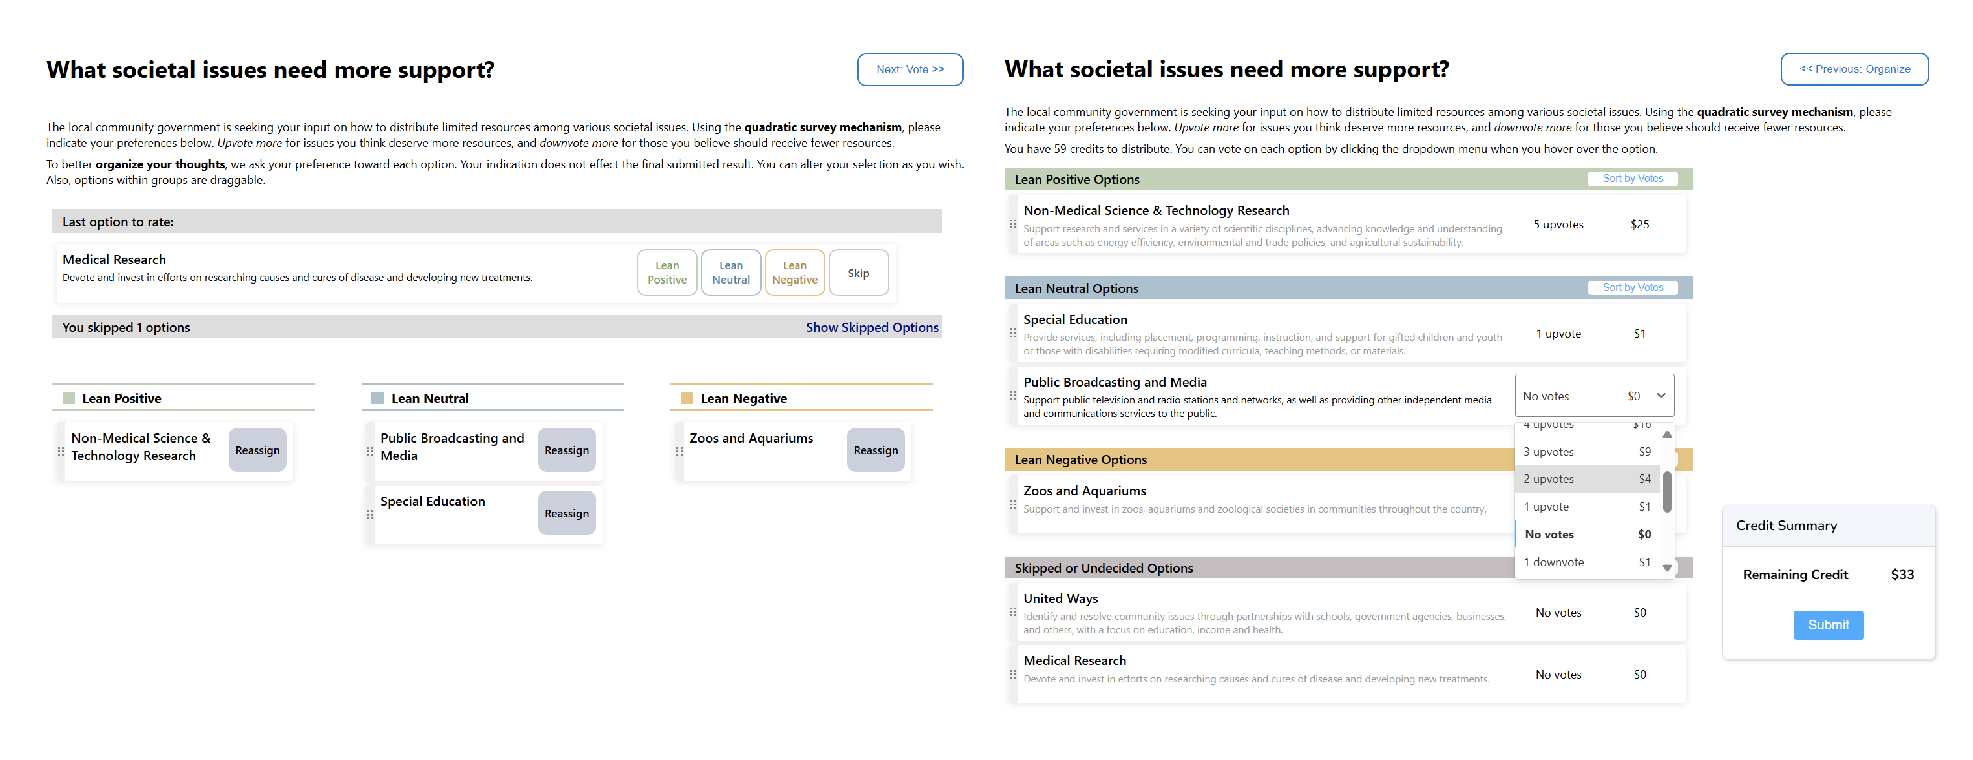
\includegraphics[width=\textwidth]{content/image/header.pdf}
    \caption{A novel two-phase interactive interface for Quadratic Surveys detailed in Sec.~\ref{sec:finalInterfaceDesign}}
    \label{fig:header}
\end{figure}

The QS and QV-like applications' capability to allow for better preference expression~\cite{chengCanShowWhat2021} across multiple options at once directly contributes to challenges such as choice overload~\cite{iyengarWhenChoiceDemotivating2000} and overchoice~\cite{gourvilleOverchoiceAssortmentType2005}. The increase in choices can raise cognitive load, leading to more frequent survey response errors and respondents opting for `good enough' rather than 'optimal' answers~\cite{lenznerCognitiveBurdenSurvey2010, blessAskingDifficultQuestions1992}. In some cases, it is impractical for decision-makers to reduce the number of options in a survey if their goal is to elicit fine-grained individual preferences simultaneously. Consequently, this research aims to examine the influence of interactive interfaces on QS at different option lengths. Thus, we seek to answer the following research questions:

\begin{itemize}
    \item RQ1. How does the number of options in QS impact respondents' cognitive load?
    \item RQ2a. How does the two-phase interactive interface influence QS respondents' cognitive load compared to a text interface?
    \item RQ2b. Across the two interfaces, what are the sources of cognitive load?
    \item RQ3. What are differences in QS respondents' behaviors when coping with long lists of options across the two-phase interactive interface and the text interface?
\end{itemize}

We designed a two-by-two between-subject in-lab study to answer these research questions. Each group of participants experienced a QS with either a short or long list of options using a text or interactive interface we designed. Participants' cognitive load was measured using NASA-TLX, followed by interviews that focused on the different elements of cognitive load. Clicksteam data was collected from participants as they completed the QS. We recruited 41 participants from a Midwestern local community, asking participants their attitudes across a wide range of societal issues. Study results analyzed and interviews are transcribe, coded, and thematically analyzed by the author.

\paragraph{Contributions}
This study introduces the first interactive interface specifically designed for Quadratic Surveys and Quadratic Voting-like applications, addressing a significant gap in existing research tools. Additionally, we conduct the first in-depth qualitative analysis which identifyed key factors contributing to cognitive load among survey respondents, leading to practical design recommendations. Although our findings did not show statistically significant differences in cognitive load as measured by NASA-TLX, our two-step interactive interface proved effective in facilitating more holistic and reflective decision-making, as evidenced by qualitative interview results. This scaffolding design promotes incremental updates and fosters deeper engagement, ultimately enhancing understanding and decision quality.

% maybe remove stat if we move to desriptive stat. Highlight first in-depth interview unserstand challegnes and explore design solutions for QM apps.

In the remainder of this paper, we focus on the related works in section~\ref{sec:relatedWorks}. Then, we detail the design decisions for the interactive QS interface, informed by the iterative design process and prior works, in section ~\ref{sec:interfaceDesign}. Experiment design follows in section~\ref{sec:experiment}. Study findings and discussion are presented in section~\ref{sec:cog_result}, section~\ref{sec:behave_result} and section~\ref{sec:discussion}.

% Some additional comments re questions
% -- does this version cut down too much?

% old tex lives here
% This challenge emphasizes the critical importance of designing and developing suitable interfaces for Quadratic Surveys to elicit truthful and in-depth preference information from respondents. Good design is essential; without it, the quality of collected data can suffer significantly. 
% These reasons strongly motivate  Addressing this question fills a important gap in the literature and enhances the practical utility of QS in capturing high-quality data across various applications.

% Highlight this is also the first work to investigate where people felt challenging when completing QS.
% At the same time, reducing cognitive load and making survey less challenging . Effective design may mitigate these overload challenges, ensuring that the Quadratic Survey mechanism fulfills its potential to capture detailed and accurate preferences. Thus, more concretely, this study focused on answering the following three research questions:

% 1. we design
% 2. we test across condition
% 3. understand what is difficult/hard through qualitative and quant responses
% --> design and usage recommendations

% Cited without details
% U.S. Colorado state government~\cite{rogersColoradoTriedNew2019}, the Democratic
%  Caucus of the House of Representatives~\cite{QuadraticVotingColorado} in the U.S., government-sponsored hackathons~\cite{teamTaiwanDigitalMinister}, and the recent Gov4git~\cite{Gov4gitDecentralizedPlatform2023}
% Despite the advocacy of Quadratic Voting by Posner and Weyl~\cite{posner2018radical}
% Political scientists have demonstrated that ballot designs alone can sway voter decisions~\cite{engstrom2020politics}, marketing and psychology researchers have examined how the presentation of questions influences responses~\cite{weijtersEffectRatingScale2010, kierujVariationsResponseStyle2010, toepoelSmileysStarsHearts2019}, and Human-Computer Interaction researchers have focused on evaluating and understanding web surveys and smart interfaces for surveys~\cite{farzandAestheticsEvaluatingResponse2024, xiaoTellMeYourself2020, pielotDidYouMisclick2024}. These studies highlight the importance of studying the interface and design for survey mechanisms.
% The Quadratic Mechanism is undeniably more complex than other voting and surveying mechanisms like the Likert scale survey~\cite{likertTechniqueMeasurementAttitudes1932}, where individuals select from a few responses, and Approval Voting~\cite{bramsApprovalVoting1978}, where participants mark as many options as they approve without constraints.

% Move this to related works.
% The effectiveness of eliciting these responses hinges upon the study protocol, survey mechanism, and design of the tool at hand~\cite{olsonWaysKnowingHCI2014, couperWebSurveyDesign2001, jackoHumancomputerInteractionHandbook2012}. While much research has explored the influence of the former two aspects, this research focuses on the design of a specific survey -- Quadratic Surveys. 

% Move this to discussion + contribution
% Thus, the primary goal of this study is to present a novel interactive interface designed for quadratic surveys, which could presumably extend to other applications that utilize the quadratic mechanism. 

% TODO, for a cleaner thesis statement in the first par? mention challenges and interface here before diving deeper.
% The importance of design in surveying tools, the growing usage of applications on the quadratic mechanism, and the lack of research on the design regarding quadratic mechanisms that one could apply, motivated our main research question: \textit{How can we design interactive interfaces to support participants in completing Quadratic Surveys?}

% Quadratic Surveys and other quadratic mechanism powered applications allow individuals 
% \begin{itemize}
% \item RQ1. How does the number of options on QS impact respondents' cognitive load?
% \item RQ2a. How does the interactive interface involving grouping and direct manipulation interface influence QS respondents' cognitive load compared to text-based interface?
% \item RQ2b. Across the two interfaces, what are the sources of cognitive load from?
% \item RQ3. What are differences in QS respondents' behaviors when coping with long lists of options?
% \end{itemize}

% Before answering these research questions, we iteratively designed and built an interactive interface informed by prior literature in the questionnaire and survey response format. Then, 